\section{Results}

\subsection{Data Imbalance}
An initial look at the data shows that there is a large number of sentences represented with values a neutral area, and very few representing the extreme cases, as shown in Figure \ref{dist:vad}.

The simplest way to initially categorise the data is to round to the nearest whole number, but as shown in Figure \ref{dist:5cat}, the extreme classes are not well represented, and would prove very difficult to train a model off. Having 5 discrete classes for each dimension also provides more detail than is probably necessary for the task at hand, so can be simplified.

\begin{figure}[h]
\centering
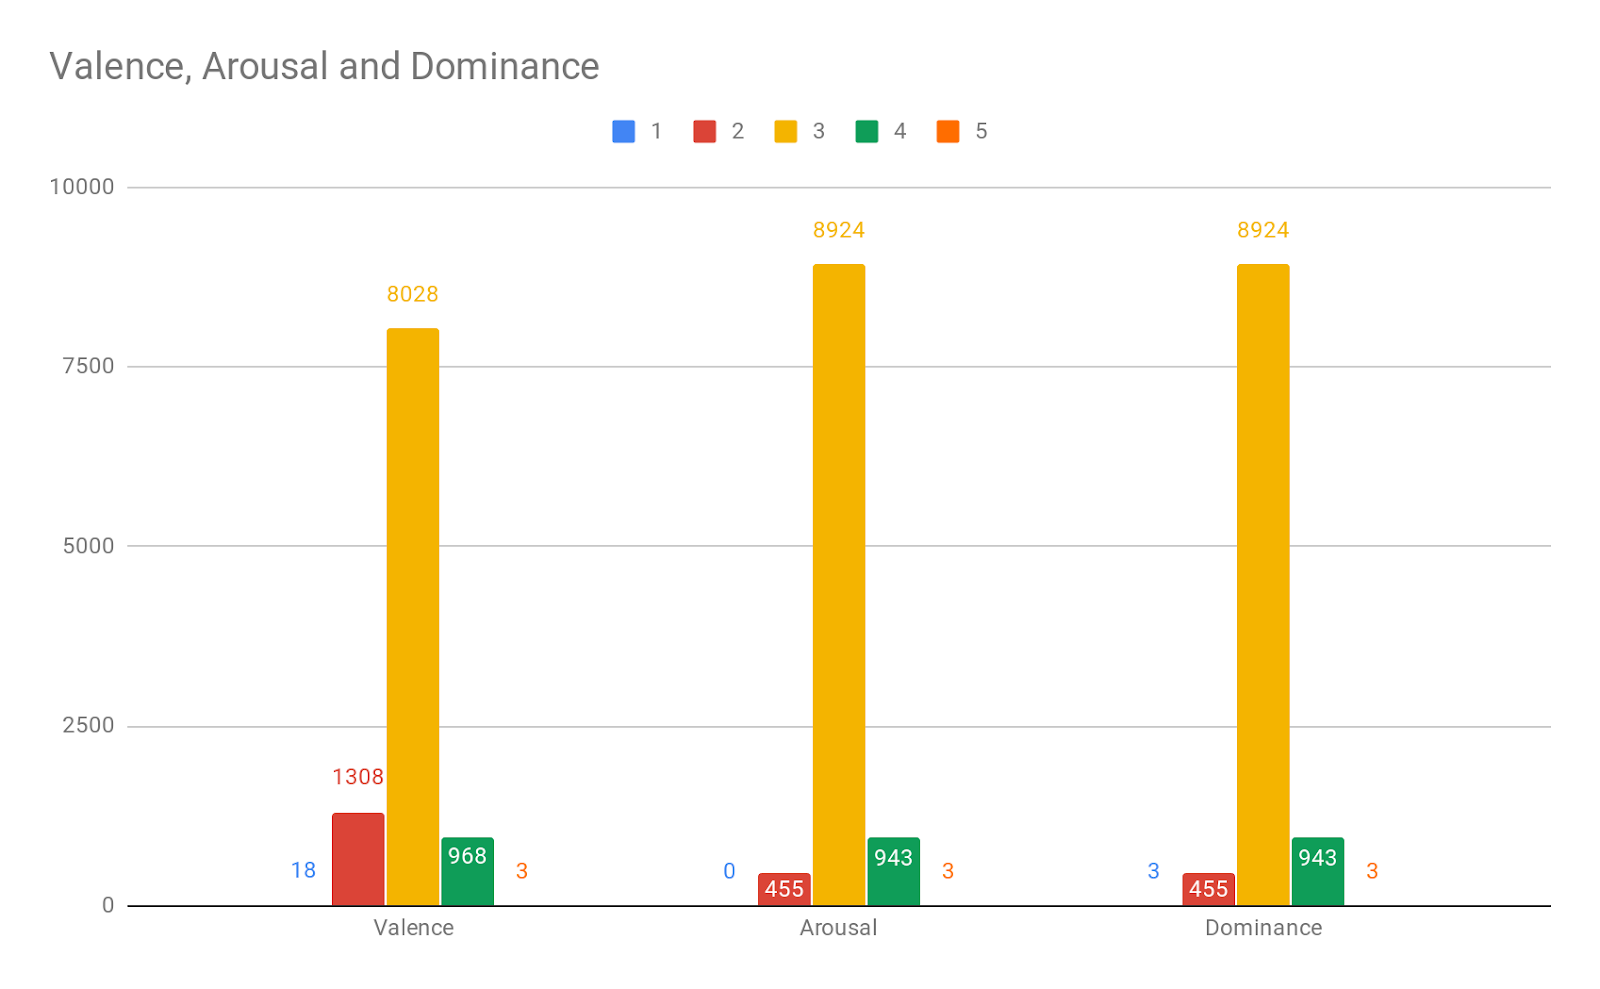
\includegraphics[scale=0.3]{graphs/5catDist.png}
\caption{Graph showing data distribution when split into five classes}
\label{dist:5cat}
\end{figure}

Splitting each dimension up into positive or negative values is also is an option, allowing an easier comparison to other work which generally does this. The issue here is that the data imbalance is still very great, particularly with the Arousal and Dominance dimensions, as shown in Figure \ref{dist:bin}.

\begin{figure}[ht]
\centering
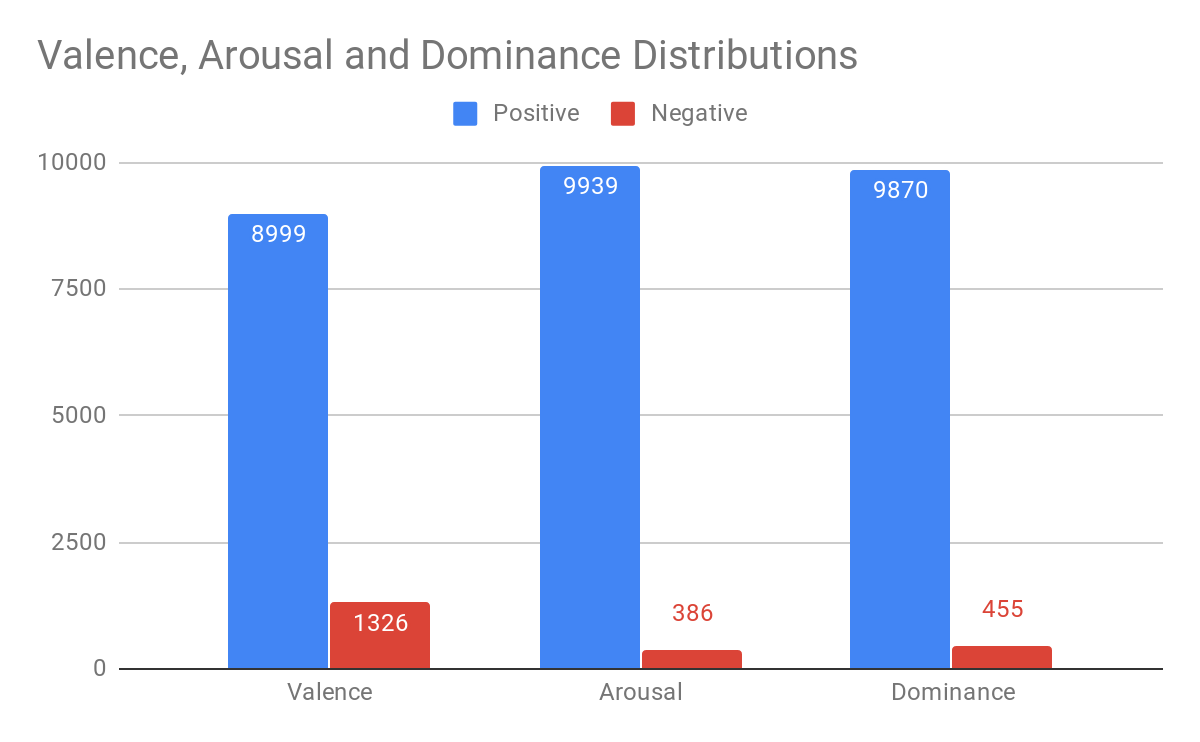
\includegraphics[scale=0.25]{graphs/binaryDist.png}
\caption{Graph showing data distribution when split into binary positive and negative classes}
\label{dist:bin}
\end{figure}

A middle ground can be found when splitting the data into positive, neutral and negative classes, as even though there is still a data imbalance there, it is less severe, and this is chosen as how to represent the data moving forward, shown in Figure \ref{dist:tri}.

\begin{figure}[H]
\centering
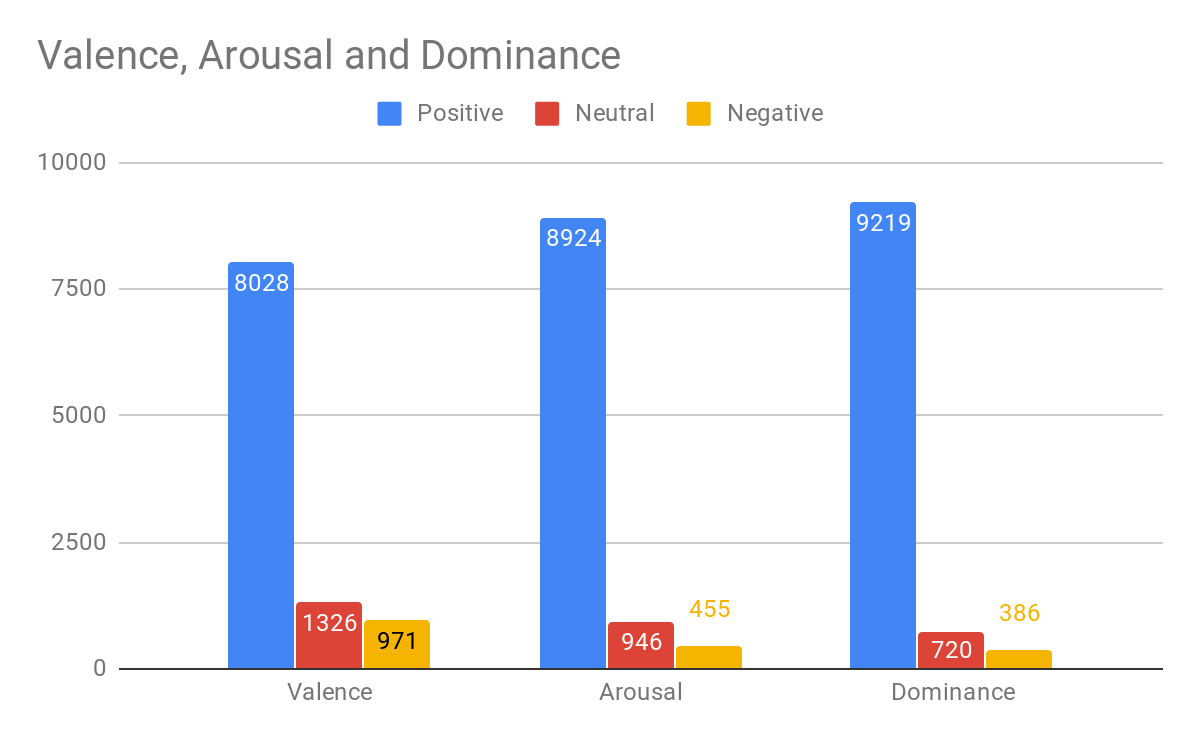
\includegraphics[scale=0.3]{graphs/nonBinaryDist.png}
\caption{Graph showing data distribution when split into positive, neutral negative classes}
\label{dist:tri}
\end{figure}

\subsection{Lexicon Anaysis}


\begin{table}
\centering
\caption{F1 scores for the 3 dimensions for the bag-of-words model}
\begin{tabular}{ |p{3cm}|p{3cm}|}
 \hline
  Dimension & F1 Score \\
 \hline
  Valence & 0.72\\
  Arousal & 0.08 \\
  Dominance & 0.80\\
 \hline
\end{tabular}
\label{lexicon:f1}
\end{table}

We can see that for the Valence and Dominance dimensions, this form of prediction performs quite well, and whether these scores can be further improved with machine learning methods will be interesting.

To explore why the Arousal dimension performs so badly, we can take a closer look at the generated confusion matrix, as shown in Table \ref{lexicon:a:conmat}. As we can see, most of the neutral data was predicted to be negative, which is definitely influenced by the trend in the bag-of-words dataset, where the average values for the Arousal are quite low. There are also no correctly predicted values in the positive class, which also contributes to the extremely low F1 score.

\begin{table}
\centering
\caption{Confusion matrix for Arousal}
\begin{tabular}{ |p{3cm}|p{3cm}|p{3cm}|p{3cm}| }
 \hline
  & \multicolumn{3}{|c|}{Predicted} \\
 \hline
   Actual & Negative & Neutral & Positive \\
    \hline
    Negative &  313   &  10  & 0 \\
    Neutral & 7001 & 384 &  3 \\
    Positive & 656 & 83 &  0 \\
 \hline
\end{tabular}
\label{lexicon:a:conmat}
\end{table}


It is also worth noting that the values in Table \ref{lexicon:a:conmat} do not cover the whole dataset either, due to instances when all of the words in the EmoBank sample cannot be found within the lexicon dataset. In this case there are around 1,500 sentences for which a VAD value could not be calculated, showing that this bag-of-words based method is far from optimal since all of the data cannot be analysed.

\subsection{Data Pre-Processing}

\begin{figure}[h]
\centering
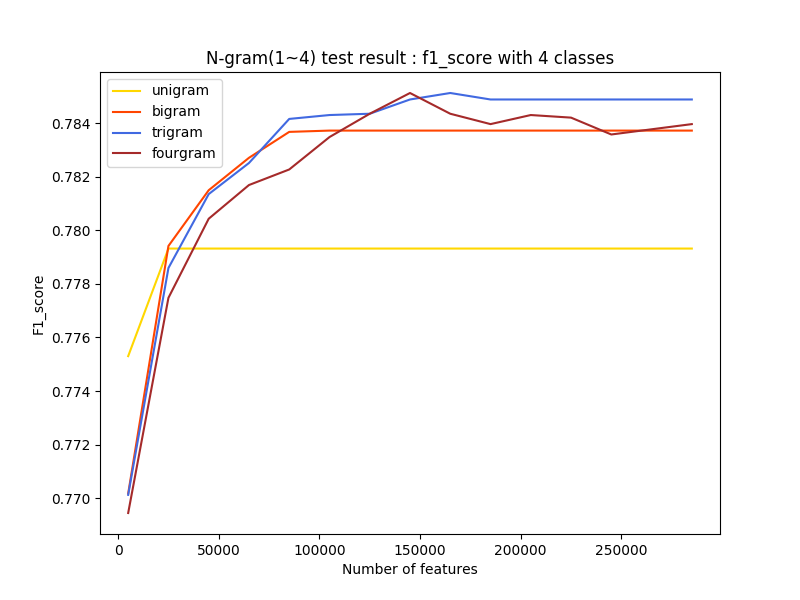
\includegraphics[scale=0.7]{graphs/nGramBinaryGraph300000.png}
\caption{Experimental Results for varying the number of features and values for N-Gram sequences}
\label{ngramGraph}
\end{figure}

As shown in Figure \ref{ngramGraph}, the F1 score improves as the N-Gram value increases up to a point, and the score also increases as the number of features does. An explanation of why the values for fourgram are generally less than for trigram, could be because the dataset is not that large and therefore predictions are less accurate as the relationships between the words cannot be properly established, so for our purposes we can leave out fourgram. It requires a significantly higher amount of processing time, as shown in Table \ref{ngram:time}. The values in Table \ref{ngram:time} are estimates calculated just to show the scale differences between the variables.

\begin{table}
\centering
\caption{Approximate Computation time for each N-Gram value.}
\begin{tabular}{ |p{3cm}|p{3cm}|}
 \hline
  N-Gram selection & Time (s) \\
 \hline
  unigram & 71\\
  bigram & 241\\
  trigram & 406\\
  fourgram & 1105 \\
 \hline
\end{tabular}
\label{ngram:time}
\end{table}
\pagebreak

\subsubsection{Hypothesis Tests}

Using the trigram values to compare, the hypothesis test shows that the F1 score still increases after 65,000 features as shown below:

$$ H_0:  \textnormal{F1 score at 65,000 features is the same than at 165,000 features (the peak on the graph)}$$

$$ H_a: \textnormal{F1 score at 65,000 features is less than at 165,000 features} $$


Using the Wilcoxon rank sum test with 95\% confidence interval p = 0.02 so reject $H_0$

But the score for F1 does not increase significantly after 85,000, which is shown as follows:

$$ H_0:  \textnormal{F1 score at 85,000 features is the same than at 165,000 features}$$

$$ H_a: \textnormal{F1 score at 85,000 features is less than at 165,000 features} $$

Using the Wilcoxon rank sum test with 95\% confidence interval p = 0.08 so reject $H_a$

We can conclude that the optimal number of features to use in the model is 85,000, since we reject the alternate hypothesis when using a hypothesis test with a 95\% accuracy if the p-value is greater than 0.05. This number of features will be used in the rest of the investigations as to maximise the score of the resultant model. 

Using this value of 85,000 features, we can compare unigram and bigram results in the following test:

$$ H_0: \textnormal{F1 score of unigram and bigram is the same at 85,000 features} $$
$$ H_a: \textnormal{F1 score of unigram is less than bigram at 85,000 features} $$

Using the Wilcoxon rank sum test with 95\% confidence interval, p = 0.01 so reject $H_0$ and accept the alternate hypothesis.

To then check bigram is the optimal, we check the F1 score does not significantly increase at 85,000 features for trigram results, so we carry out the following test:

$$ H_0: \textnormal{F1 score of bigram and trigram is the same at 85,000 features} $$
$$ H_a: \textnormal{F1 score of bigram is less than trigram at 85,000 features} $$

Using the Wilcoxon rank sum test with 95\% confidence interval p = 0.10 so reject $H_a$.

So we can conclude using bigrams is optimal for processing the data for inputting into the model.

The R scripts for running these tests are referenced in Appendix \ref{appendix:hypothesis}.

\subsection{Model Selection}


\begin{figure}[h]
\centering
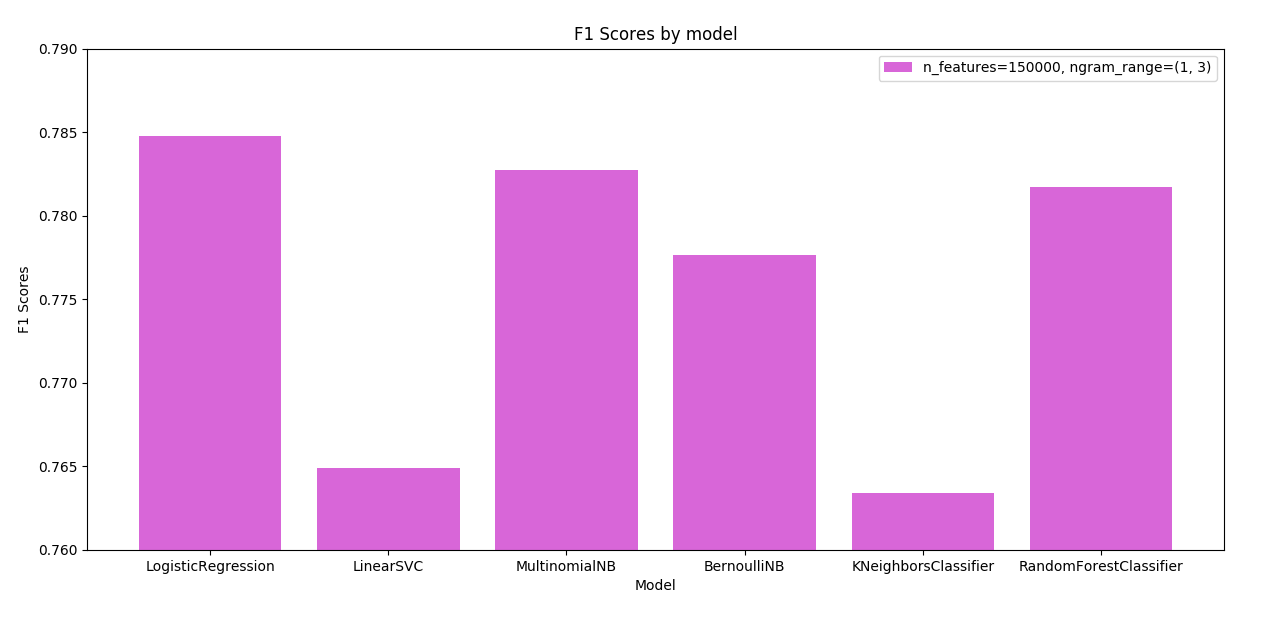
\includegraphics[scale=0.5]{graphs/models.png}
\caption{Graph showing the different F1 scores for varying types of classifier}
\label{model:graph}
\end{figure}

The inbuilt models in the sklearn package with default settings were used for initial comparison, and as we can see from Figure \ref{model:graph} the difference between the models is very slight, with the F1 scores all within a 3\% range of score. Since each of the models compared are all using their default settings within the sklearn package, more work could be done to optimise them further in the future, but just to argue for choosing the best default classifier the following hypothesis test is run.

\subsubsection{Hypothesis Tests}

We can see that out of the three top models, two of the classifiers that were expected to perform well, Logistic Regression and Multinomial Naive Bayes do so, as well as the Random Forest Classifier. We can prove by hypothesis tests with 95\% confidence interval for a two sided Wilcoxon rank sum test that these three can all be classed as the same. To further compare these three models then, we can look at how long it takes for each fold to train and test each model. These tests can be found in Appendix \ref{appendix:hypothesis}.

\begin{table}
\centering
\caption{F1 scores for the 3 dimensions for machine learning model}
\begin{tabular}{ |p{3cm}|p{3cm}|}
 \hline
  Classifier & Average time per fold (s)\\
 \hline
  Logistic Regression & 1.80\\
  Multinomial Naive Bayes & 0.51 \\
  Random Forest & 3.04\\
 \hline
\end{tabular}
\label{model:times}
\end{table}

We can see from Table \ref{model:times} that the Multinomial Naive Bayes Classifier takes a much shorter time to run, so we can select this as the optimal model to use.

\subsection{Sampling methods}

We can see from the results from the investigation shown in  Figure \ref{oversamplegraph}, using any of the oversampling methods decreases the F1 score by a significant amount. 

\begin{figure}[ht]
\centering
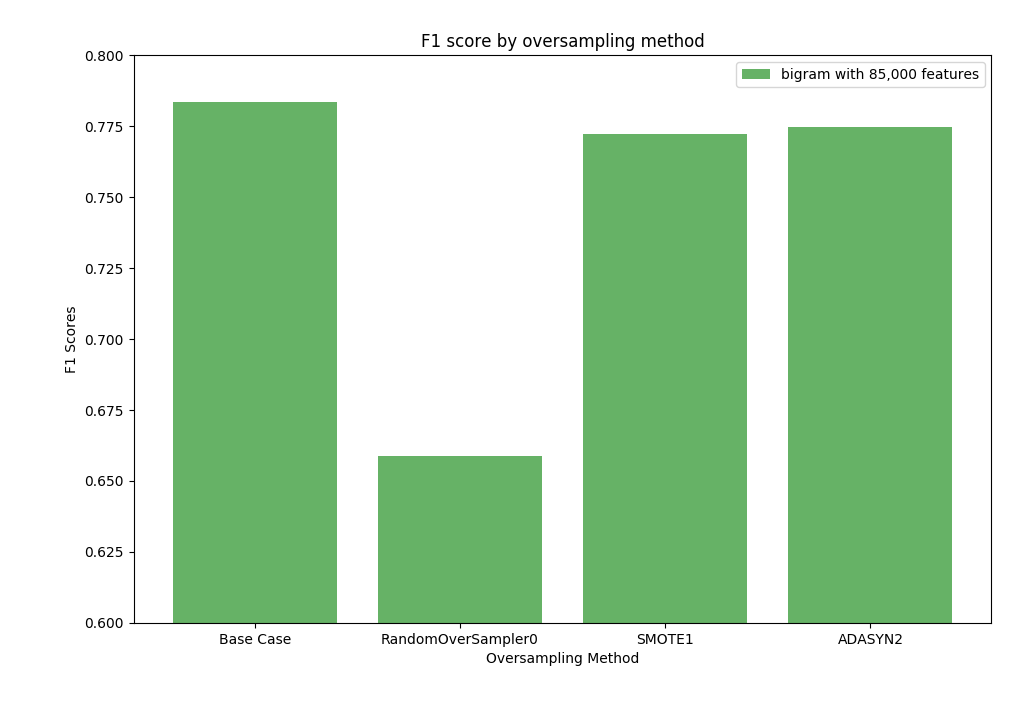
\includegraphics[scale=0.5]{graphs/OversampleNB.png}
\caption{Graph showing the F1 score for different oversampling methods}
\label{oversamplegraph}
\end{figure}

An explanation as to why this is happening is most likely a combination of using textual data, which is known to cause issues with oversampling methods, and the severity of the imbalance in the data. In the valence class, which is the one we are analysing at this point, the negative samples make up less than 10\% of the overall data and therefore many of the synthetic samples that are created will not make grammatical sense and be of poor quality. 

To ensure that the base case is higher than the second highest result, the ADASYN sampler we run a hypothesis test as follows:

$$ H_0: \textnormal{F1 score of the base case and ADASYN is the same} $$
$$ H_a: \textnormal{F1 score of the base case is greater than ADASYN} $$

Using the Wilcoxon rank sum test with 95\% confidence interval p = 8.98E-5 so reject $H_0$. So we can conclude that using no oversampling methods leads to the highest F1 score.


The undersampling methods were known to not give promising results, but due to the issues with oversampling over such a large class imbalance, briefly investigating this was something that could potentially have worked, but as the experimental results shown in Figure \ref{undersamplegraph}, they all made the model perform significantly worse or did not work at all and hence can be disregarded. The near miss undersampling methods did not work as it could not maintain the quality of data while reducing the majority classes to the size of the minority classes, the minority classes were just too small.

\begin{figure}[ht]
\centering
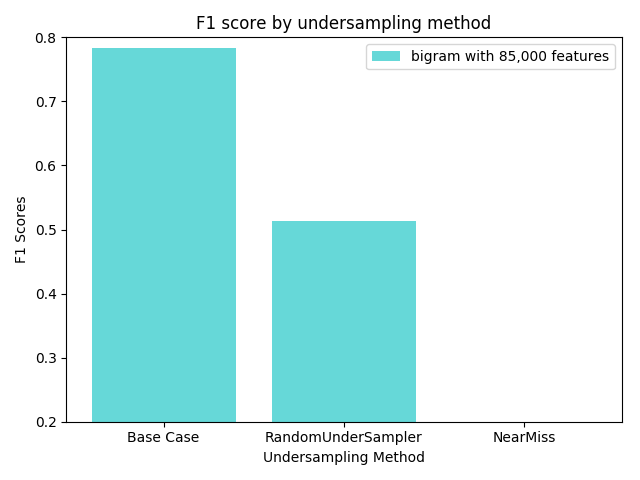
\includegraphics[scale=0.6]{graphs/undersampleNB.png}
\caption{Graph showing the F1 score for different undersampling methods}
\label{undersamplegraph}
\end{figure}

\subsection{Final Model}
\label{finalModelSection}
The final model that was produced then had the following characteristics: 

\begin{itemize}
    \item The data was formatted into bigram "words".
    \item The most frequent 85,000 n-gram "words" were used as input features.
    \item The classification model is Multinomial Naive Bayes.
    \item No oversampling or undersampling techniques were applied.
\end{itemize}

This results in a model that has the F1 scores for the prediction of each dimension shown in Table \ref{ML:f1}.

\begin{table}
\centering
\caption{F1 scores for the 3 dimensions for machine learning model}
\begin{tabular}{ |p{3cm}|p{3cm}|}
 \hline
  Dimension & F1 Score \\
 \hline
  Valence & 0.78\\
  Arousal & 0.86 \\
  Dominance & 0.89\\
 \hline
 Average & 0.843\\
 \hline
\end{tabular}
\label{ML:f1}
\end{table}

\subsection{Implementation}

A decision was made to not show the user the VAD values, and just the result song to begin with. After the users reaction to the response song has been assessed, the calculated Ekmans emotion can be shown.

\begin{figure}[ht]
\centering
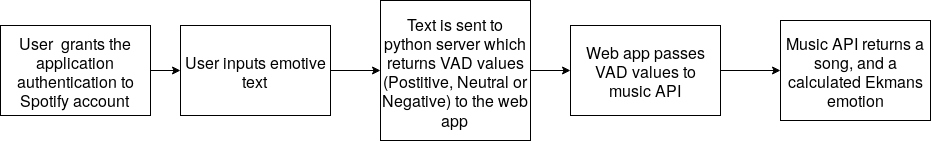
\includegraphics[scale=0.6]{litImgs/interfaceFlow.png}
\caption{User activity through the application}
\label{implementationFlow}
\end{figure}

\begin{figure}[ht]
\centering
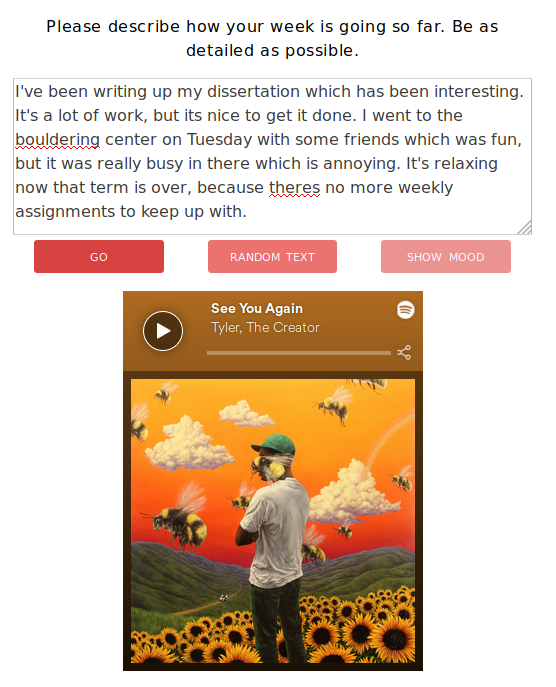
\includegraphics[scale=0.4]{implementation/tamara.png}
\caption{Layout of main UI page}
\label{UIlayout}
\end{figure}

Getting an F1 score of 0.84 on the model is a reasonable result, but testing whether users believe that the model is accurately predicting their moods is something that needs to be assessed. Using the built web application on conjunction we are able gain feedback from test users, asking them to input their own text and access their own Spotify data through the application to obtain a result.

Out of the 5 users that the program was tested with, 3 concluded that the song did match their emotion and 2 did not. This is a very small focus group, and for a more detailed analysis more feedback needs to be gathered, but for the purpose of gaining insight into whether the system is appropriate for answering the research question, an initial idea can be obtained.

It was decided to initially hide the calculated Ekmans emotion from the user, so that their analysis of the result song is not influenced. 
Two users, one which agreed with the result and one that did not are studied in more detailed as follows:

\subsubsection{User A}

\begin{figure}[h]
\centering
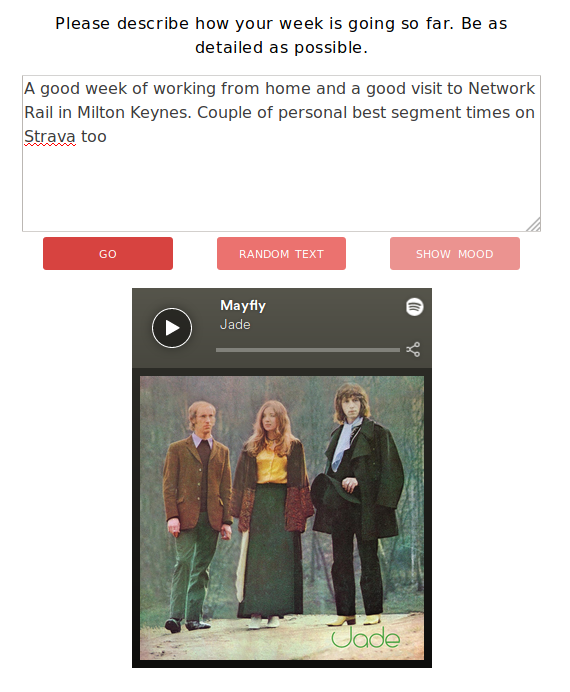
\includegraphics[scale=0.4]{implementation/malc-user.png}
\caption{User A: input and output}
\label{user:1}
\end{figure}

The first user concluded that the song matched what they had input, stating that it was upbeat and had "positive vibes". They did suggest that it would be nice to see how the song was calculated in more detail however. The calculated Ekman's emotion in this case was "Surprise", which was decided was incorrect, particularly when knowing that "Happy" was one of the options that could have been selected.

\begin{table}[h]
\centering
\begin{tabular}{|l|l|}
\hline
 Valence &  0.7\\
 Arousal &  0.6\\
 Domiance &  0.5\\
 Ekman's Emotion &  Surprise\\ \hline
\end{tabular}
\end{table}

\pagebreak

\subsubsection{User B}

\begin{figure}[h]
\centering
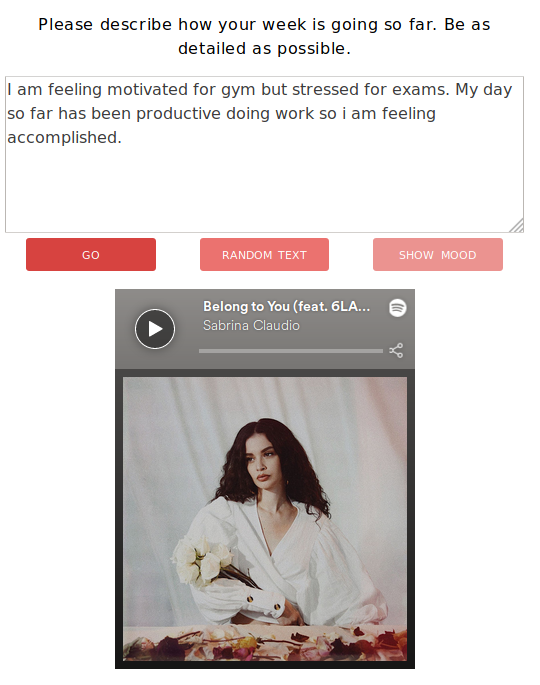
\includegraphics[scale=0.4]{implementation/jana.png}
\caption{User B: input and output}
\label{user:2}
\end{figure}

The second user concluded that the song did not match their mood, since its a very relaxed song, but they did mention that they've been listening to a lot of relaxing music recently. Other reasons why the song did not fit were also discussed, such as words such as "exams" and "work" potentially having an effect on the result. Looking more at the song data behind why this result would have been incorrect, the data Spotify allocated to the song rates it with a high danceability of 0.6, although User 2 disagrees with this. An explanation for this result may be that the Spotify data is not the most accurate, but this is is quite subjective.

\begin{table}[h]
\centering
\begin{tabular}{|l|l|}
\hline
 Valence &  0.6\\
 Arousal &  0.6\\
 Domiance &  0.5\\
 Ekman's Emotion &  Surprise\\ \hline
\end{tabular}
\end{table}

All but 2 of the tests gave the result Ekman's emotion back as "Surprise", and the other two came back with "Disgust" which was incorrect every time. An explanation for these results would be because of the way that the data has been split up into discrete classes the 3D distance between the points.